\cleardoublepage
\chapter{Experiments and Results}
\label{chap:experiments}

%Introduce Chapter: 3 experiments (test set size = 3) to test the whole
%shape matching methodology. Its separated in three main processes: initial
%processing, automatic shape matching and manual fixing. The results are 
%presented and discussed.

In this chapter the different experiments carried out to test the performance
of the shape matching solution are 
presented, explaining the reason for their choice and the test objectives.
Then the results are presented and discussed, pointing out the advantages and drawbacks of the suggested
shape matching model, that are infered from the first ones.

\section{Experiments}
\label{sec:experiments}

In order to test the implemented solution, three digital images of worms in liquid
media where selected from the image database of the Department of Bioscience and Nutrition
of the \emph{Karolinska Institute}. Each image corresponds to a different difficulty level, 
following the criteria of number of worms and degree of overlap. Thus the greater the number 
of worms in the image and the greater the number of worms that are connected by overlapping,
the greater the difficulty level. The overlapping degree is determined by the number
of worms that belong to the different \emph{worm clusters} (first defined in Sec. \ref{sec:reasoning})
and the number of \emph{worm clusters} in the image.
The selected images are named \emph{test image 1}, \emph{test image 2} and \emph{test image 3}
and are disposed in an increasing difficulty level order, from the easiest to the hardest. 
Below in Table \ref{tab:testset} the characteristics of the test set are presented.


\begin{table}[h]
  \caption{Test set images characteristics}
\begin{center}
\begin{tabular}[h]{|>{\columncolor[gray]{0.9}} p{2cm} |p{3cm} | p{2.8cm} | p{3cm}| p{2.8cm} |}
    \hline
    \rowcolor[gray]{.9}
    Test Image& Number of Isolated Worms & Number of Worm Clusters & Number of Worms per Clusters  & Total Number of Worms\\
    \hline
    Test 1 & 11/19 (57.8\%) & 3 & 8/19 (42.1\%) & 19 \\
    \hline
    Test 2 & 8/33 (24.2\%) & 3 & 25/33 (75.7\%)& 33 \\    
    \hline
    Test 3 & 13/38 (34.2\%)& 5 & 25/38 (65.7\%) & 38 \\
    \hline 
  \end{tabular}
\end{center}
  \label{tab:testset}
\end{table}


For each test image a series of experiments were carried out to test the performance of
the different processes that are involved in the solution methodology. The entire 
shape fitting process was divided into three stages that represent the 
main fitting steps. These are: \emph{Initial Processing}, \emph{Automatic Shape Matching} and
\emph{Matching Manual Fixing}.\\

The \emph{Initial Processing} involves all the image processing steps that are performed 
before the shape matching optimization process, as explained in Sec.\ref{sec:solmet},
such as: thresholding, distance transformation, skeletonization, 
clustering, endpoint detection and worm profiling. Among these, the distance transformation
and skeletonization follow already implemented and tested algorithms (covered in Sec.\ref{sec:metdt}
and Sec.\ref{sec:metsk}) and produce straight forward results, so there is no need to make further analysis
about them.
The clustering process follows the skeletonization process and is straight forward as well.
On the other hand the thresholding, endpoint detection and worm profiling processes vary 
from image to image, so different experiments are carried out in order to test these subprocesses
for the test set.\\

The \emph{Automatic Shape Matching} stage consists in experiments dealing with the automatic
optimization process to match \emph{worm clusters} and contour following technique to match 
\emph{isolated worms} that produce a first fitting guess for the worms in the image. These 
experiments attempt to measure the efficacy and time efficiency of different variations of the
matching algorithm, in order to conclude about properties of the algorithm and the feasibility 
of the automatic solution.\\
The third stage,\emph{Matching Manual Fixing}, attempts to measure the type and amount of 
manual modification operations that must be performed by the user in order to fix the 
matchings that were wrongly assigned by the automatic process. The experiment is also 
aimed to determine how much can the efficacy of the automatic solution be improved, in
order to get a better matching. Once the best possible matching is found through manual fixing,
a distribution of the matching energies is presented, that aimes to study the sensitivy of the
matching algorithm. This consist on a graph showing the best three conformations, in terms of the objective
function, starting from every endpoint, comparing how far are the top two conformations from
the right one.\\

The experiments were executed in a personal computer with a 2.00 GHz AMD Turion 
Dual-Core Mobile Processor,1 MB Microprocessor chace and 3Gb of RAM Memory, 
on Linux Operating System, Ubuntu Distribution.

\section{Results}
\label{sec:results}

In this section the results obtained for the test set are presented and discussed. The results are distributed in the three main stages: \emph{Initial Processing}, \emph{Automatic Shape Matching} and
\emph{Matching Manual Fixing}. In the section \emph{Initial Processing} the results for the three different 
images in the test set are presented. On the other hand the section \emph{Shape fitting} presents the different
results for the stages \emph{Automatic Shape Matching} and \emph{Matching Manual Fixing} for every test image
individually.

\subsection{Initial Processing}
\label{sec:initproc}

This section presents the results for the experiments carried out over the test set for the 
processes: thresholding and endpoint finding. Then a brief discussion about
the result for the worm profiling process is also presented.

\subsubsection*{Thresholding}

As explained in Sec.\ref{sec:thresimp} \emph{Endrov} has implementations for the 
thresholding filters \emph{Fukunaga},\emph{Max entropy}, \emph{Otsu} and \emph{Percentile}.
The process to determine that a binary image represents sufficiently well the original 
image was done by visual appreciation. In order to select an appropriate thresholding
filter, the four previously mentioned were tried on every test image, tweaking the
input parameters until the best possible binary image was obtained from every one.
It resulted that among the four methods, the \emph{Percentile} filter generated the
best binary images for the three tests. The next closer method was \emph{Fukunaga}
that produced acceptable solutions after the combination of binary images
generated from different number of classes, however the results were not as good as
the ones obtained with \emph{Percentile}, requiring more processing as well.\\

Following this experiment the \emph{Percentile} method was selected by being considered
sufficiently good to generate a binary representation for the worms in the image 
and easy to manipulate. Below in table \ref{tab:threshold} the best percentile 
values for every test image are presented.


\begin{table}[h]
  \caption{Best percentile value for Percentile Thresholding for test image}
\begin{center}
\begin{tabular}[h]{|>{\columncolor[gray]{0.9}} c |c|c|c|}
    \rowcolor[gray]{.9}
    \hline
    Test & Test Image 1 & Test Image 2 & Test Image 3\\
    \hline
    Percentile Value & 0.074 & 0.1 & 0.11\\
    \hline
  \end{tabular}
\end{center}
  \label{tab:threshold}
\end{table}

The resultant best percentile values oscillate between $0.074$ and $0.11$, and are 
simple to determine using \emph{Endrov}.   

\subsubsection*{Endpoint detection}

Once the process of skeletonization is performed the worm endpoints are detected
in the image by finding the extreme skeleton points. Starting from these the 
skeleton is expanded following the directional neighbor process explained in
Sec.\ref{sec:wend} until contour points are found. These contour points will
correspond to worms endpoints.\\
As explained, worm endpoints are detected by first identifying extremes in the worm
skeleton. However when the extreme of a given worm in an image overlaps with 
another worm shape, the binary image will consider this worms as part of the 
same shape and in consequence the shape skeleton will generate a continuous 
path and not an extreme skeleton point, thus the endpoint will not be detected.\\
Since the solution methodology is centered on finding paths between endpoints and 
then determining the most likely worm paths, having missing endpoints would
affect greatly the matching accuracy, as it is shown later in the subsections 
\emph{Automatic Shape Matching} for every test image results.\\

Since the worm endpoints are simple to determine visually, a manual process
of adding and removing pixel operations can be performed fastly in order to
add the missing endpoints and disconnect them from the rest of skeleton, as
explained in Sec.\ref{sec:endpointop}.
The removing operation is required because by definition a worm endpoint 
belongs to a extreme of the skeleton and then only one directional 
path should be able to start from it, \emph{i.e.}a worm endpoint has only
one \emph{cardinal neighbor} belonging to the skeleton.
As described in Sec.\ref{sec:endpointop},
the process consists basically on selecting a skeleton pixel that is not marked as
endpoint and then selecting the wrong skeleton neighbor pixel to disconnect the path 
from the wrong part of the skeleton. \\

Below, Table \ref{tab:endtable} presents the number of endpoints identified
automatically for ever test image and the number of operations that must be
performed to fix the missing endpoints. An operation corresponds to the combination
of an add/remove pixel operation.


\begin{table}[h]
  \caption{Worm endpoints detection and fixing for the test set}
\begin{center}
\begin{tabular}[h]{|>{\columncolor[gray]{0.9}} p{2cm} |p{1.9cm}|p{2cm}|p{2.2cm}|}
    \rowcolor[gray]{.9}
    \hline
    Test Image & Total Endpoints & Detected Endpoints & Add/Remove Operations\\
    \hline
    Image 1 & 38 & 38 (100\%) & 0 \\
    \hline 
    Image 2 & 66 & 53 (80\%) & 13 \\
    \hline 
    Image 3 & 76 & 57 (75\%) & 19 \\
    \hline
  \end{tabular}
\end{center}
  \label{tab:endtable}
\end{table}

From the table above, it can be infered that a high number of worms belonging
to \emph{worm clusters} increases the chances to have endpoints overlapping, 
as well as it does a higher number of worms in total in the same space.
Considering the high amount of worms that belong to worm clusters 
for images two and three ($75\%$ and $65\%$ respectively) and the few
amount of clusters for each one (which increases the overlapping) the amount
of missing endpoints can be considered fairly low, and is feasible in time 
to fix them manually.

\subsubsection*{Worm Profiling}

In order to generate an accurate worm profile of the worms present in the image
it is necessary to have \emph{isolated worms} in the processing image. The percentage 
of \emph{isolated worms} for every image were $57.8\%$, $24.2\%$ and $34.2\%$ 
respectively,
oscillating between $8$ and $13$ worms, as shown in Table \ref{tab:testset}. 
For all of this images the generated worm profiles were sufficiently accurate to
conduct the optimization shape matching process, whose results are presented in 
the subsections named \emph{Automatic Shape Matching} of every test image results.

\subsection{Shape Matching}

In this section the results for the second and third stage in the 
solution methodology are presented, as described above in Sec. \ref{sec:experiments}, which consist
in \emph{Automatic Shape Matching} and \emph{Matching Manual Fixing}. 
For the \emph{Automatic Shape Matching} subsection the results for a series of four 
variations of the matching algorithm are presented, focusing on the matching accuracy 
and time performance. The two main variations are: Path Guessing and Every Path. 
Path Guessing is the version of the algorithm in which every guessed path is favored
by an improvement in its shape optimization value, by reducing it to the half. So when 
a conformation is to be chosen for an endpoint the value of the guessed path is more likely
to be selected. On the other hand, the Every Path variation does not consider the 
path guessing but all the possible conformations for every endpoint.
Each of this variations are executed with and without adding the missing endpoints. So the
four variations are: Every Path (missing endpoints), Path Guessing (missing endpoints), 
Every Path and Path Guessing. These last two contain all the endpoints of the image.\\

The \emph{Matching Manual Fixing} presents the results of modifying the erroneous matches
obtained by the best automatic matching algorithm, showing the resulting best
possible matching image and indicating the number of worm shapes that had to be 
re-arranged. This process is done manually: The user detects the wrong matching visually 
and selects two endpoints to obtain the best optimized shape that connects them, as
explained in Sec. \ref{sec:matchfix}. An operation (as used in the tables for this section) 
is considered to be the process of selecting two endpoints and generate a new shape.\\

Then a subsection \emph{Matching Energy} is presented in which the distribution of
the energy values for the different conformations is discussed. This sections presents
a graph showing the different energy values (objective function) for the correct conformation
and the next two best conformations for every endpoint (of those having three or more conformations). 
The correct conformation corresponds to that one that is constructed between the two endpoints that
belong to the worm in the image. The other two are conformations that start in the
selected endpoint and end in a wrong one.


\subsubsection*{Automatic Shape Matching (Test Image 1)}

Since for the test image 1 all the endpoints are found automatically, as shown in 
Table \ref{tab:endtable}, the results presented here show the matching efficacy and
runtime just for the variations Every Path and Path Guessing, that include all the
worm endpoints. Below Table \ref{table:auto1} presents the obtained results.

\begin{table}[h]
  \caption{Results of automatic worm shape matching on test image 1}
  \begin{center}
  \begin{tabular}{|>{\columncolor[gray]{0.9}} p{3cm}|p{2.8cm}|p{2.8cm}|p{2.8cm}|c|}
    \hline
    \rowcolor[gray]{.9}
    Path finding & Isolated Worms matching & Cluster Worms matching 
    & Total Matching 
    & Time (s) \\ 
    \hline
    Every Path & 11/11 (100\%) & 6/8 (75\%) & 17/19 (89.5\%)& 6.47 \\
    \hline
    P.Guessing & 11/11 (100\%) & 8/8 (100\%) & 19/19 (100\%) & 7.53 \\
    \hline
  \end{tabular}
\end{center}
  \label{table:auto1}
\end{table}

It can be observed that in both variations of the algorithm the 
\emph{isolated worms} were all matched. For the worms that belong 
to clusters, the Every Path variation matched correctly $6/8$ corresponding
to the $75\%$ of the clustered worms, for a total matching of $17/19$. On 
the other hand the Path Guessing variation managed to match automatically 
all the worms in the image. The execution time is slightly higher for the
Path Guessing Variation, as expected because of the extra calculations that
must be performed to calculate the best paths departing from each endpoint.\\

For this image, the Path Guessing variation represented an improvement in 
the solution, by inducing the shape produced from guessed paths to be more
likely to be selected. On the other hand, at first glance, the isolated
worms seem to be matched regardless of the algorithm variation, as expected.\\
Below in Fig.\ref{fig:best1} the best matching for test image 1, corresponding to the Path Guessing variation, is shown.


\begin{figure}[h!]
  \centering
  \subfloat[Best Match]{\label{best1}\includegraphics[scale=0.42]{results/test1/complete-frame1}}
\qquad
  \subfloat[Best Match over original image]{\label{bestbg1}\includegraphics[scale=0.42]{results/test1/complete-framebg1}}
  \caption{Best automatic shape matching on test image 1}
  \label{fig:best1}
\end{figure}


\subsubsection*{Automatic Shape Matching (Test Image 2)}

Below in Table \ref{tab:tab2} the results for automatic matching on test image
2 are shown, presenting the previously mentioned variations of the
matching algorithm: Every Path and Path Guessing, with and without missing
points. The abbreviation \emph{me}, next to the variation name, means 
\emph{missing endpoints}.

\begin{table}[h]\begin{tabular}{|>{\columncolor[gray]{0.9}} p{3cm}|p{2.8cm}|p{2.8cm}|p{2.8cm}|c|}
    \hline
    \rowcolor[gray]{.9}
    Path finding & Isolated Worms matching & Cluster Worms matching 
    & Total Matching 
    & Time (s) \\ 
    \hline  
    Every Path (me) & 8/8 (100\%) & 7/25 (28\%) & 15/33 (45.4\%) & 21.8 \\ 
    \hline
    P.Guessing (me) & 8/8 (100\%) & 10/25 (40\%) & 18/33 (54.5\%) & 23.7\\
    \hline
    Every Path & 8/8 (100\%)& 15/23 (65.2\%) & 23/33 (69.7\%)& 42.3 \\
    \hline
    P.Guessing & 8/8 (100\%)& 21/25 (84\%) & 29/33 (87.8\%) & 45 \\
    \hline
  \end{tabular}
  \label{tab:tab2}
  \caption{Results of automatic worm shape matching on test image 2}
\end{table}

It can be observed that for every variation the Isolated Worms where matched
totally. For the two variations that have missing endpoints just around
the half of the total worms could be matched. Though the execution time is
lower, which is expected given the decrease of feasible paths, not having an
endpoint of a worm makes impossible to find a shape that matches it correctly.
For the variations that include endpoints the results are better showing 
$69.7\%$ and $87.8\%$ percentage of total matching for Every Path and 
Path Guessing respectively. \\
It can be observed that the Path Guessing variation
increases the matching accuracy considerable, in both missing and not missing
endpoints set of variations. The execution time also increases considerably
for the set of variations that contain all the endpoints, as expected. 
The Path Guessing variation presents just a slight execution time increase with
respect to the Every Path, while increasing the matching percentage 
considerably.\\
In the best case the automatic matching solution manages to fit the shape
for all the isolated worms and $84\%$ of the clustered worms, for 
a total matching of $87.7\%$ in $45$ seconds.

\subsubsection*{Matching Manual Fixing (Test Image 2)}

The Path Guessing with no missing endpoints variation resulted to be the 
best one, with just four worms wrongly matched among thirty three. The 
resulting image was selected to fix the wrong assignations and obtain
the best match as possible.
Below Fig.\ref{fig:best2} presents four images. The first two correspond to the
best automatic solution, previously mentioned, without and with the original
image as background. The next conserve the same pattern but show the manual
fixed image.

\begin{figure}[h!]
  \centering
  \subfloat[Best Automatic Match]{\label{best1}\includegraphics[scale=0.5]{results/test2/guessing-nobgframe}}
\qquad
  \subfloat[Best Automatic Match over original image]{\label{bestbg1}\includegraphics[scale=0.5]{results/test2/guessing-bgframe}}
\qquad
  \subfloat[Manual Fixed Match]{\label{bestbg1}\includegraphics[scale=0.5]{results/test2/frame2-allnobg}}
\qquad
  \subfloat[Manual Fixed Match over original image]{\label{bestbg1}\includegraphics[scale=0.5]{results/test2/frame2-all}}

\caption{Best automatic shape matching and Manual match fixing on test image 3}
\label{fig:best2}
\end{figure}


The manual fixing required 4 operations consisting in selecting two
endpoints that correspond to an actual worm shape. After selected the
endpoints the assigned shapes starting at this endpoints are removed
and the best shape that connects the two selected endpoints is added.
After the manual fixing the $100\%$ of the worms in the image could 
be fitted.


\subsubsection*{Automatic Shape Matching (Test Image 3)}

Below in Table \ref{tab:tab3} the results for automatic matching on test image
3 are presented. The four variations for the algorithm are shown.
 The abbreviation \emph{me}, next to the variation name, means 
\emph{missing endpoints}.

\begin{table}[h]\begin{tabular}{|>{\columncolor[gray]{0.9}} p{3cm}|p{2.8cm}|p{2.8cm}|p{2.8cm}|c|}
    \hline
    \rowcolor[gray]{.9}
    Path finding & Isolated Worms matching & Cluster Worms matching 
    & Total Matching 
    & Time (s) \\ 
    \hline  
    Every Path (me) & 13/13 (100\%) & 5/25 (20\%) & 18/38 (47.3\%) & 26.4 \\ 
    \hline
    P.Guessing (me) & 13/13 (100\%) & 7/25 (28\%) & 20/38 (52.6\%) & 28.7\\
    \hline
    Every Path & 13/13 (100\%)& 13/25 (52\%) & 26/38 (68.4\%)& 36.2 \\
    \hline
    P.Guessing & 13/13 (100\%)& 16/25 (64\%) & 29/38 (76.3\%) & 39.8 \\
    \hline
  \end{tabular}
  \label{tab:tab3}
  \caption{Results of automatic worm shape matching on test image}
\end{table}

For every variation the isolated worms where all matched successfully.
For the first two variations: Every Path and Path Guessing with missing points, 
the total matching is around the half of the total. 
The next two variations, that do
not have missing endpoints, increase the level of accuracy considerable,
reaching $68.4\%$ and $76.3\%$ for Every Path and Path Guessing, respectively.\\
The all-endpoints variation set show a considerable increase in the
execution time with respect to the missing endpoints one. 
The Path Guessing variations present a increase in the matching accuracy
in both cases, as well as a slight increase in execution time.\\
The best variation was the Path Guessing with no missing endpoints, managing
to match all the \emph{isolated worms} and a total of $76.3\%$ of the 
whole image.

\subsubsection*{Matching Manual Fixing (Test Image 3)}

The Path Guessing with no missing endpoints variation resulted to be the 
best one, with nine worms wrongly matched among thirty eight. The 
resulting image was selected to fix the wrong assignations and obtain
the best match as possible.
Below Fig.\ref{fig:best3} presents four images. The first two correspond to the
best automatic solution, previously mentioned, without and with the original
image as background. The next conserve the same pattern but show the manual
fixed image.

\begin{figure}[h!]
  \centering
  \subfloat[Best Automatic Match]{\label{best1}\includegraphics[scale=0.42]{results/test3/guess-nobg}}
\qquad
  \subfloat[Best Automatic Match over original image]{\label{bestbg1}\includegraphics[scale=0.42]{results/test3/guess-bg}}
\qquad
  \subfloat[Manual Fixed Match]{\label{bestbg1}\includegraphics[scale=0.42]{results/test3/all-nobg}}
\qquad
  \subfloat[Manual Fixed Match over original image]{\label{bestbg1}\includegraphics[scale=0.42]{results/test3/all-bg}}
  \caption{Best automatic shape matching and Manual match fixing on test image 3}
  \label{fig:best3}
\end{figure}


The manual fixing required 9 operations to fix the incorrectly matched worms.
After the fixing process, the $100\%$ of the worms in the image could be
matched and fitted.
\subsection{Matching Energy}

In this section the matching energy distribution is presented 
for every test image, using a graph. 
Every graph consists in a series of endpoints in the
x axis, and energy values in the y axis. For each endpoint three values 
are given that correspond to the correct conformation and the best two 
conformations that are not the correct one. The correct conformation
is such that a shape is constructed starting from the endpoint in the
x axis and reaching another endpoint that corresponds to an actual
worm in the image. The next two conformations also start from the x axis
endpoint but reach an incorrect endpoint, thus they do not represent 
actual worms.\\
For each test image the graph is presented and discussed, focusing 
on the accuracy level of energy value given to the correct conformation
and its correspondence to the other two values. The correct conformation
is traced with blue squares (connected by a blue line) while the next two
are traced in red and green respectively.\\
It is important to recall that the energy formulation function, covered
in Sec.\ref{sec:clusterfit}, evaluates the distance between a matching shape
and a matched shape as the percentage of background pixels contained in the 
area covered by the matching shape, so all the possible energy values are
contained in the interval $[0,1]$ and the optimized shapes tend to take values
from one to three decimals close to $0$.

\subsubsection*{Test Image 1}

Below in Fig.\ref{fig:energy1} the best matching energy values for 
test image 1 are presented.

\begin{figure}[h]
 \centering
   \includegraphics[scale=0.9]{results/test1/energy-graph}
 \caption{Energy value for the best three conformations by endpoint on test
image 1. The selected endpoints correspond to worms in worm clusters that
have more than two possible conformations}
\label{fig:energy1}
\end{figure}

In the graph can be observed that for most endpoints the correct conformation
resulted to be also the one with lowest energy value, thus representing
the best matching distance between the optimizing shape and the original shape.
For two cases a wrong conformation had a lower energy value that the correct
one, meaning that 
although the conformation is not correct the matching objective function
considers the shape more likely to be an accurate worm shape that the right
one. For all the cases the conformation with the second lowest value, was
clearly worst than the correct conformation, thus the accuracy level given
by the energy value for the correct conformation corresponds to what it is 
expected.\\

\subsubsection*{Test Image 2}

In Fig.\ref{fig:energy2} the best matching energy values for 
test image 2 are presented. For this case there are shown energy values
for twenty nine endpoints.

\begin{figure}[h!]
 \centering
   \includegraphics[scale=0.9]{results/test2/energy-graph}
 \caption{Energy value for the best three conformations by endpoint on test
image 2. The selected endpoints correspond to worms in worm clusters that
have more than two possible conformations}
\label{fig:energy2}
\end{figure}

It can be observed that the second best conformation (in green) is in all 
the cases worst that the best conformation, normally from two to four times 
in terms of the energy function value, thus the correct conformation is 
either the best or the second best conformation, from all the possible.
In this case only four endpoints among twenty nine show a better energy
function value for the best next conformation (in red) over the correct 
conformation (in blue). This coincides directly with the results shown
in Table \ref{tab:tab3} where, for the best automatic solution (Path Guessing),
the amount of worms successfully matched was 29/33, which is only four worms
away from the optimal solution, the same number of endpoints in which the
correct conformation is not the best in value. In fact, the difference of 
values between the correct and best next conformation for the these four
endpoints is close enough to think that a more sensitive objective function
could retrieve the correct conformation for all the cases for the automatic
algorithm.\\ 

\subsubsection*{Test Image 3}

Below in Fig.\ref{fig:energy3} the best matching energy values for 
test image 3 are presented.

\begin{figure}[h]
 \centering
   \includegraphics[scale=0.9]{results/test3/energy-graph}
 \caption{Energy value for the best three conformations by endpoint on test
image 3. The selected endpoints correspond to worms in worm clusters that
have more than two possible conformations}
\label{fig:energy3}
\end{figure}

In the figure can be observed that among the twenty two endpoints, for nine
of them the second best conformation resulted to have a better energy value
than the correct conformation. This is consistent with the results presented
in Table \ref{tab:tab3} where for the best variation (Path Guessing), the
number of wrongly detected worms is also nine. This means that an incorrect 
path is considered to be more likely to be a worm starting from this
endpoints. For every endpoint,with the exception of one, the second best 
solution is worst than the correct solution. So the energy value of the 
correct solution is either the best or the second best.\\

Given that for this image the amount of worms that belong to clusters
is high (25), is easy to observe that the amount of possible paths starting
from every endpoint is increased and so is the amount of wrong conformations.
As explained, for this image, nine of twenty two endpoints had wrong 
conformations with the lowest energy value, thus the energy formulation 
is not sensitive enough in this cases. However the difference between
the correct and selected conformations for these cases is close (just as
for test image 2), so a more sophisticated objective function could lead
to better results.\\

In this section the matching results for the three test images were given. 
The three main stages concerning the shape fitting process: 
\emph{Initial Processing}, \emph{Automatic Shape Matching} and 
\emph{Matching Manual Fixing}, were tested thoroughly in order to observe and
study the behavior of the whole worm fitting methodology proposed in this
work. In the next chapter the conclusions taken from the result chapter are
addressed, as well as  some future work suggestions.



